\section{Các linh kiện sử dụng}
Để tạo nên mạch điện tử, không thể thiếu những linh kiện cơ bản. Trong mục này, chúng ta sẽ liệt kê và mô tả các thành phần chính được sử dụng trong dự án.

\begin{itemize}
    \item \textbf{Điện trở:} Điện trở được sử dụng để hạn chế dòng điện trong mạch, giúp bảo vệ các thành phần nhạy cảm khỏi hư hỏng gây ra bởi dòng điện quá mức.

    \begin{figure}[h!]
        \centering
        % Ảnh trái
        \begin{subfigure}{0.5\textwidth}
            \centering
            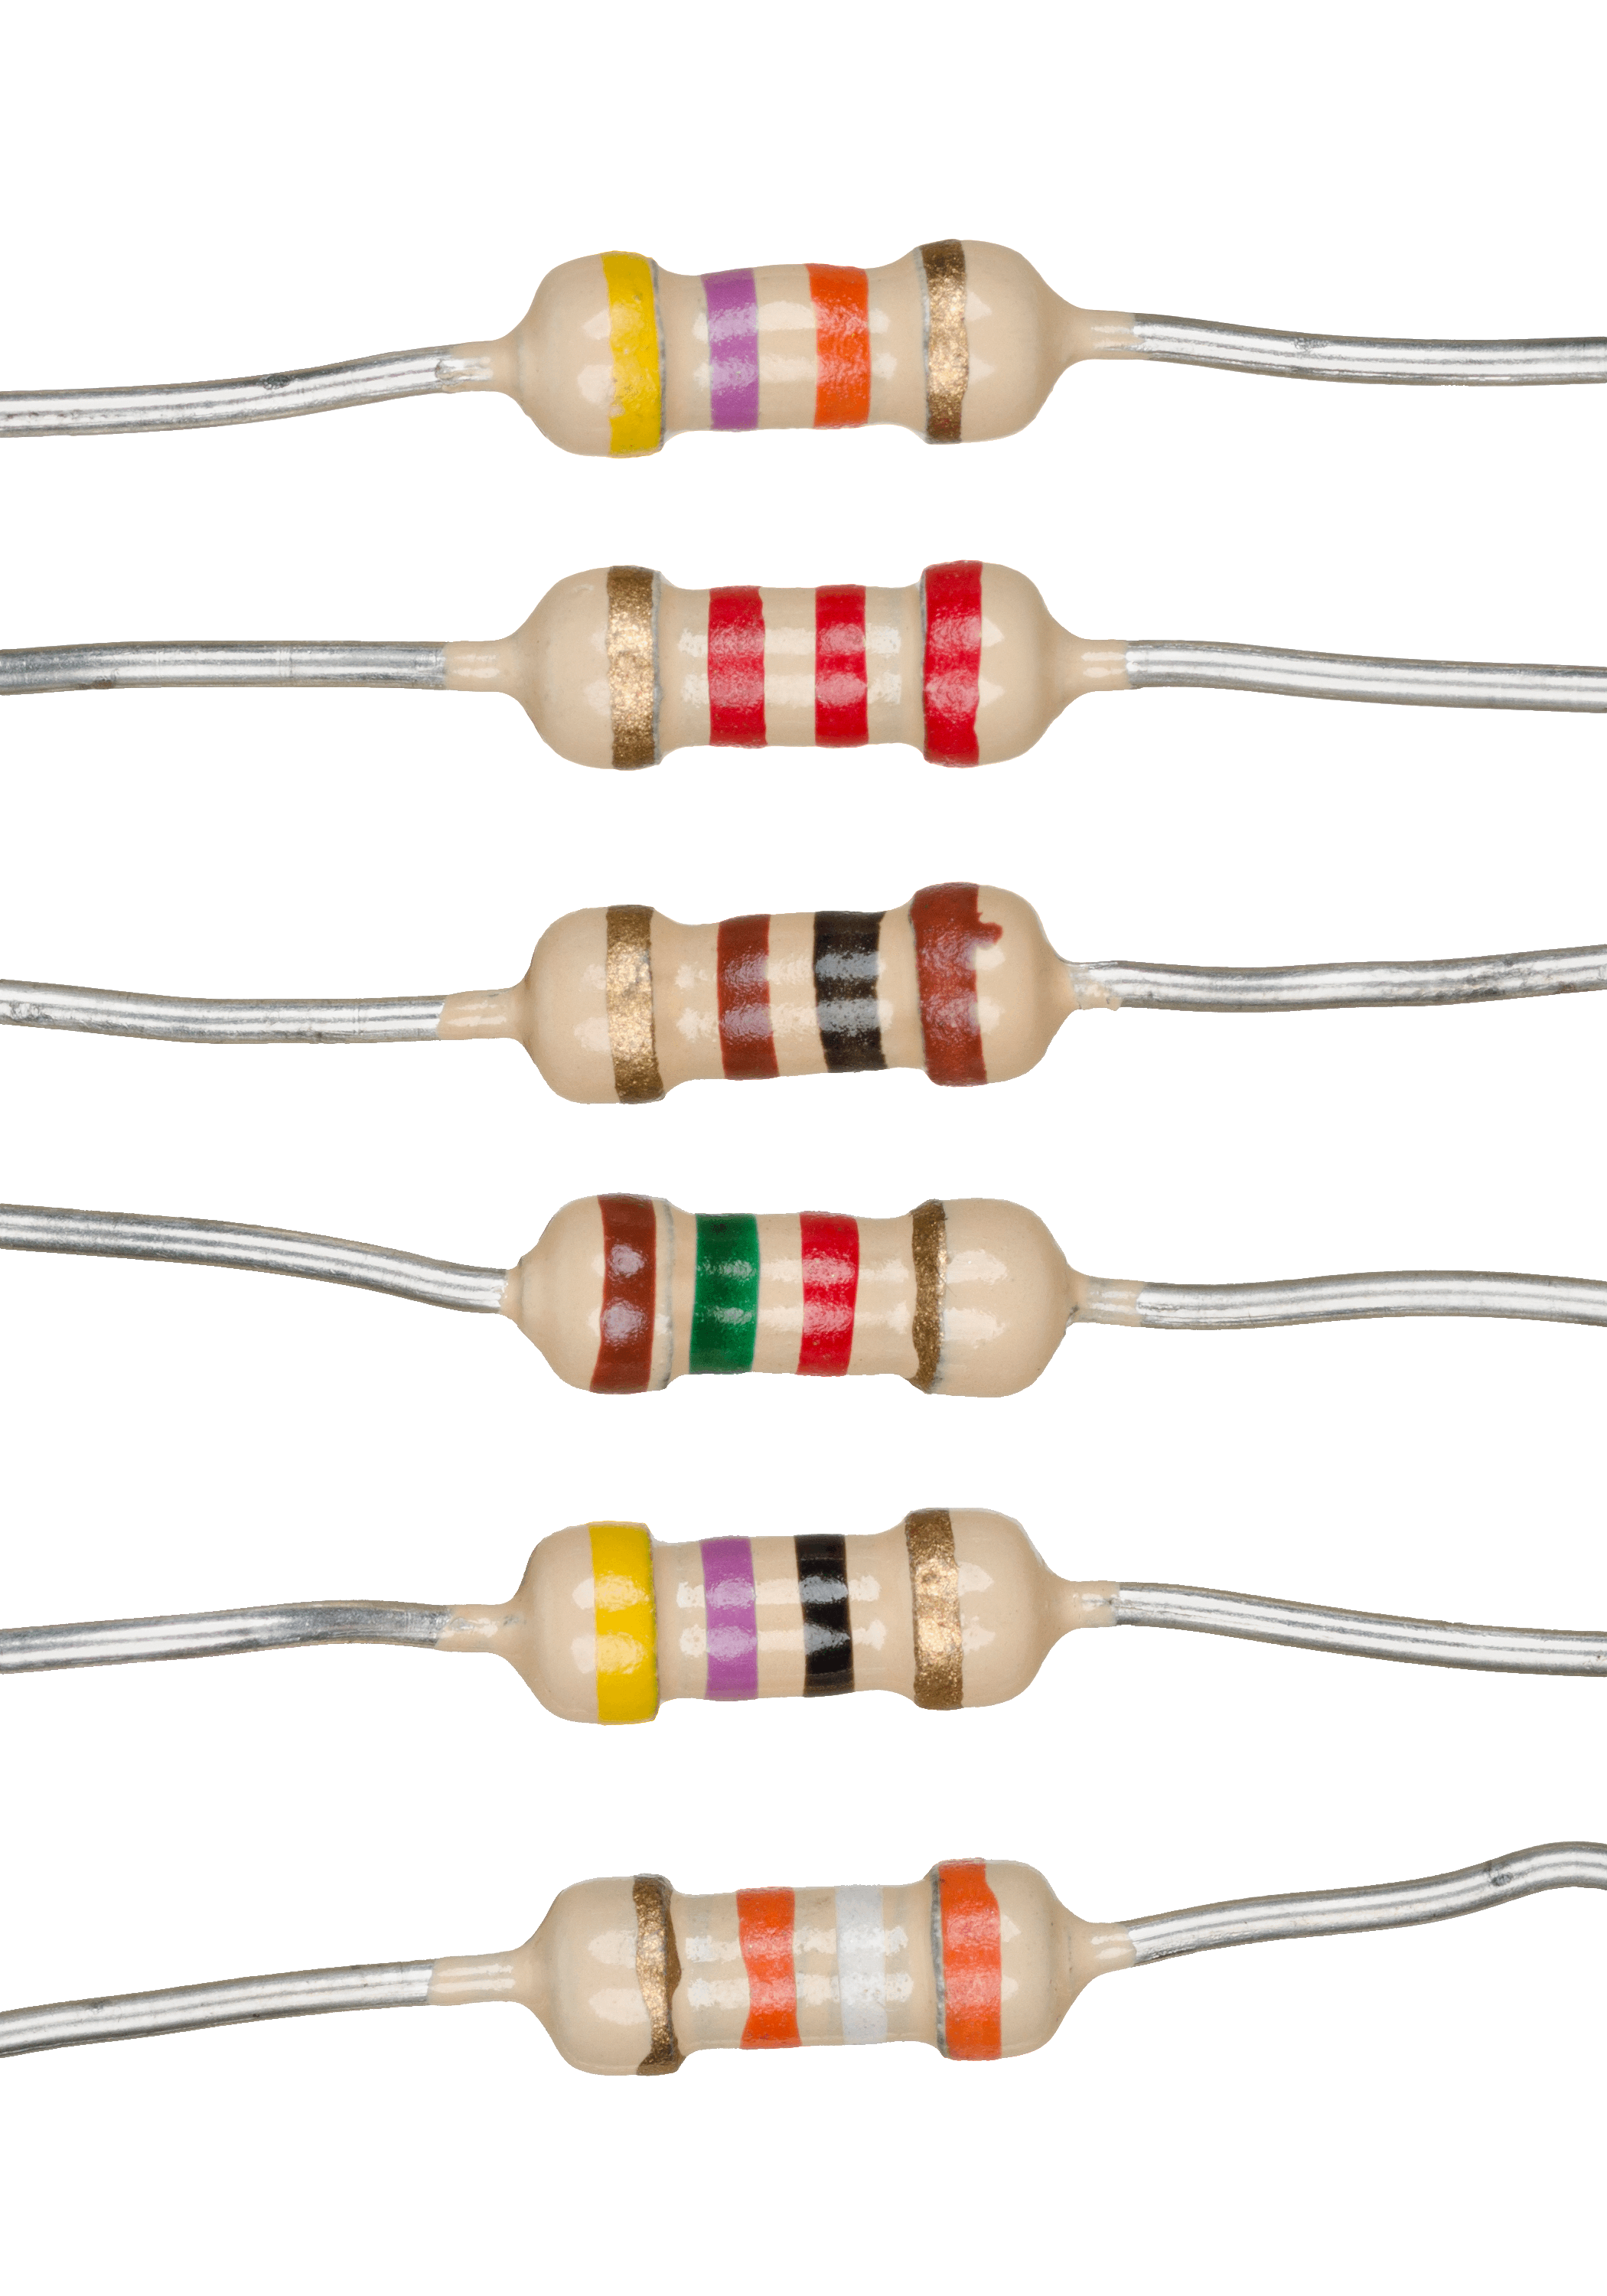
\includegraphics[width=0.3\textwidth]{graphics/section2/resistors.png}
            \caption*{Điện trở}
        \end{subfigure}
        \hfill
        % Ảnh phải
        \begin{subfigure}{0.45\textwidth}
            \centering
            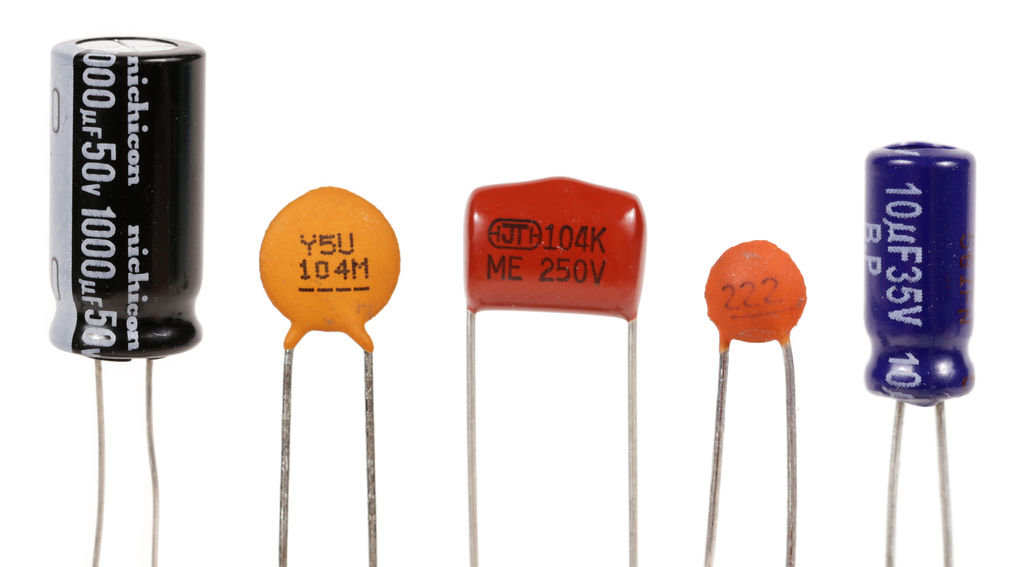
\includegraphics[width=\textwidth]{graphics/section2/capacitors.png}
            \caption*{Tụ điện}
        \end{subfigure}
        \caption*{}
    \end{figure}
    \item \textbf{Tụ điện:} Tụ điện lưu trữ và giải phóng năng lượng điện. Tụ điện có tác dụng khử nhiễu và ổn định điện áp trong mạch điện.

    \item \textbf{Cuộn cảm:} Cuộn cảm lưu trữ năng lượng trong từ trường khi có dòng điện chạy qua. Chúng được sử dụng trong các ứng dụng lọc và lưu trữ năng lượng.
    \begin{figure}[h!]
        \centering
        % Ảnh trái 
        \begin{subfigure}{0.5\textwidth}
            \centering
            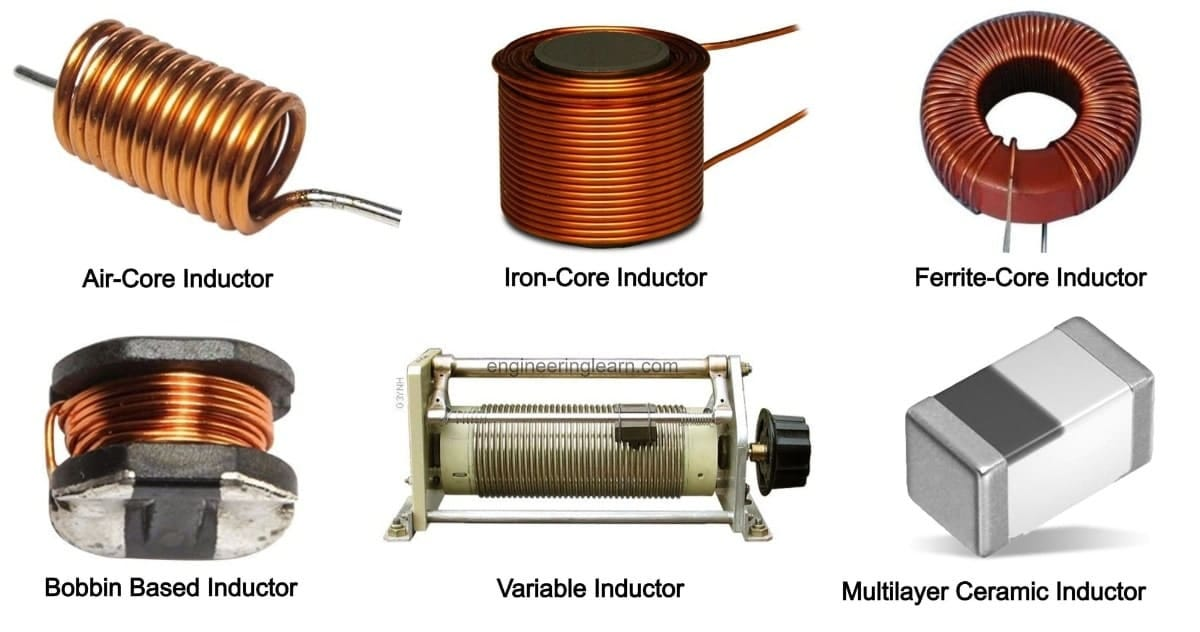
\includegraphics[width=\textwidth]{graphics/section2/inductors.png}
            \caption*{Cuộn cảm}
        \end{subfigure}
        \hfill
        % Ảnh phải
        \begin{subfigure}{0.45\textwidth}
            \centering
            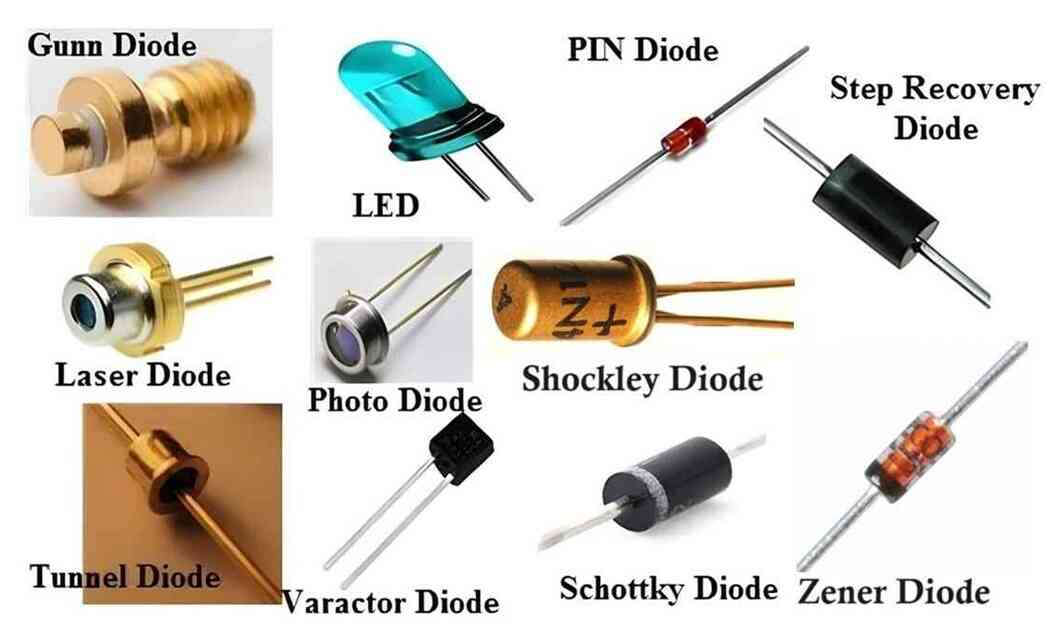
\includegraphics[width=\textwidth]{graphics/section2/diodes.png}
            \caption*{Các loại diode}
        \end{subfigure}
        \caption*{}
    \end{figure}
    \item \textbf{Diode:} Nhờ dặc tính cho phép dòng điện chạy theo một hướng duy nhất của mình, diode được dùng phổ biến nhất trong việc bảo vệ mạch khỏi dòng điện ngược.
    \bigskip
        \item \textbf{Transistor:} Transistor được sử dụng để khuếch đại và chuyển mạch. Chúng là các khối xây dựng cơ bản trong các mạch điện tử hiện đại.
    
        \begin{figure}[h!]
            \centering
            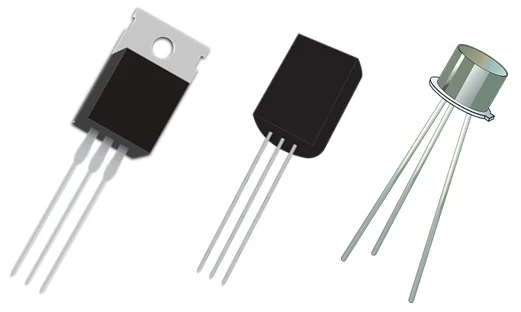
\includegraphics[width=0.5\textwidth]{graphics/section2/transistors.png}
            \caption*{Một số loại transistors}
        \end{figure}
    
        \item \textbf{Mạch tích hợp (IC - Integrated Circuit):} Một số IC được sử dụng trong dự án với các đặc điểm và ứng dụng chính:
        \begin{itemize}
            \item \textbf{IC LM358:} tích hợp 2 con OpAmp (bộ khuếch đại thuật toán). Nó được sử dụng để khuếch đại tín hiệu trong mạch.
            
            \begin{figure}[h!]
            \centering
            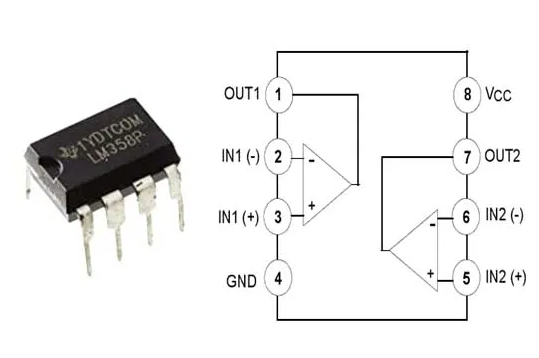
\includegraphics[width=0.5\textwidth]{graphics/section2/IC_LM358.png}
            \caption*{IC LM358}
        \end{figure}

        \item \textbf{IC MAX485:}là IC giao tiếp chuyên dụng để chuyển đổi tín hiệu UART sang tín hiệu RS- 485, một giao thức truyền thông nối tiếp được sử dụng rộng rãi. Với đặc tính tiêu thụ năng lượng thấp và khả năng truyền dữ liệu lên đến 10 Mbps, MAX485 phù hợp cho các hệ thống giao tiếp trong môi trường công nghiệp hoặc đường truyền dài.
           \newpage
        \begin{figure}
                \centering
                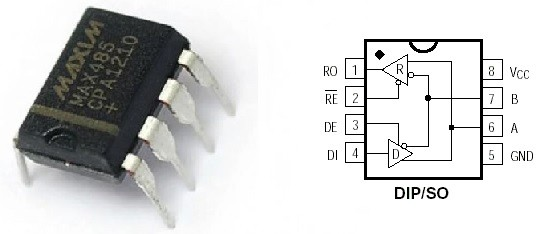
\includegraphics[width=0.5\textwidth]{graphics/section2/IC_MAX485.png}
                \caption*{IC MAX485}
        \end{figure}
            
            
        \item \textbf{TSP5430:} TSP5430 là một bộ chuyển đổi DC-DC giảm áp (step-down converter) với khả năng hoạt động ở dải điện áp đầu vào rộng từ 5.5V đến 36V. Trong mạch của dự án, nó được dùng để cung cấp nguồn điện 3.3V.
        \begin{figure}[h!]
            \centering
            % Ảnh trái 
            \begin{subfigure}{0.49\textwidth}
                \centering
                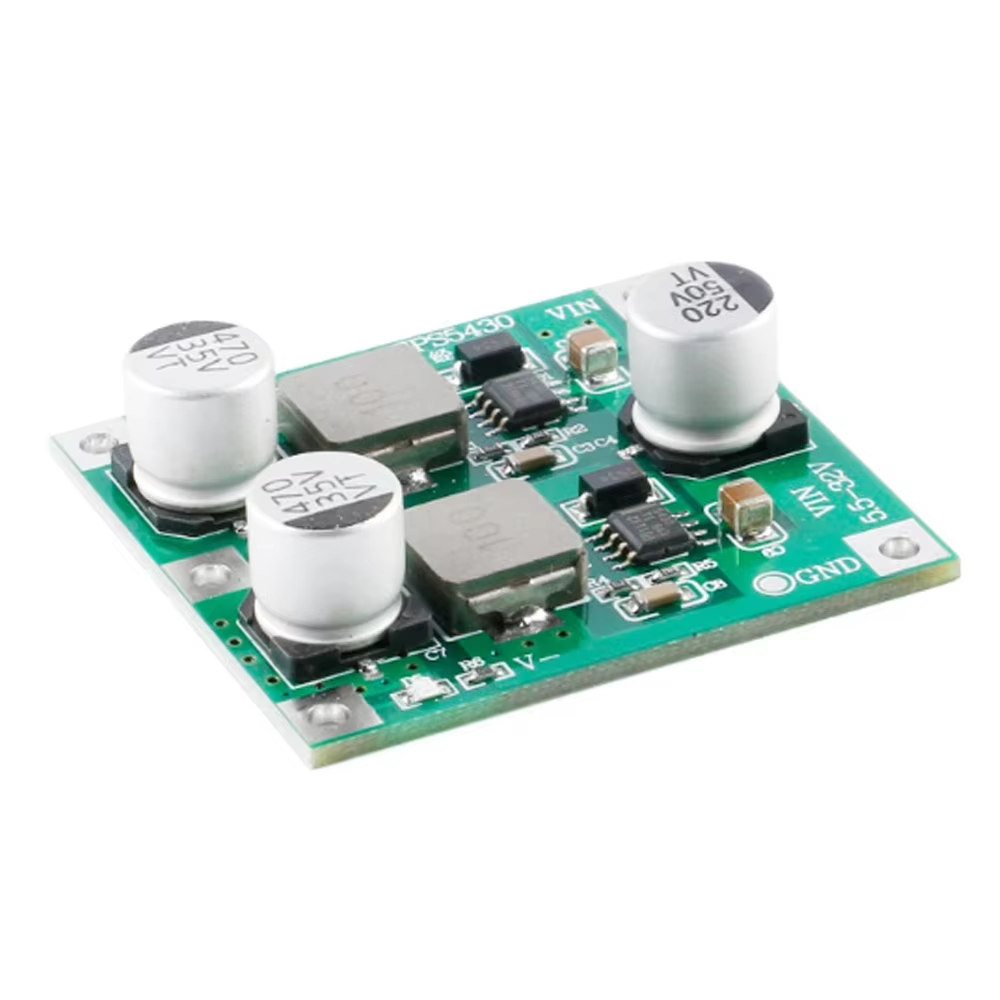
\includegraphics[width=\textwidth]{graphics/section2/TPS5430.png}
                \caption*{Mạch TSP5430}
            \end{subfigure}
            \hfill
            % Ảnh phải
            \begin{subfigure}{0.49\textwidth}
                \centering
                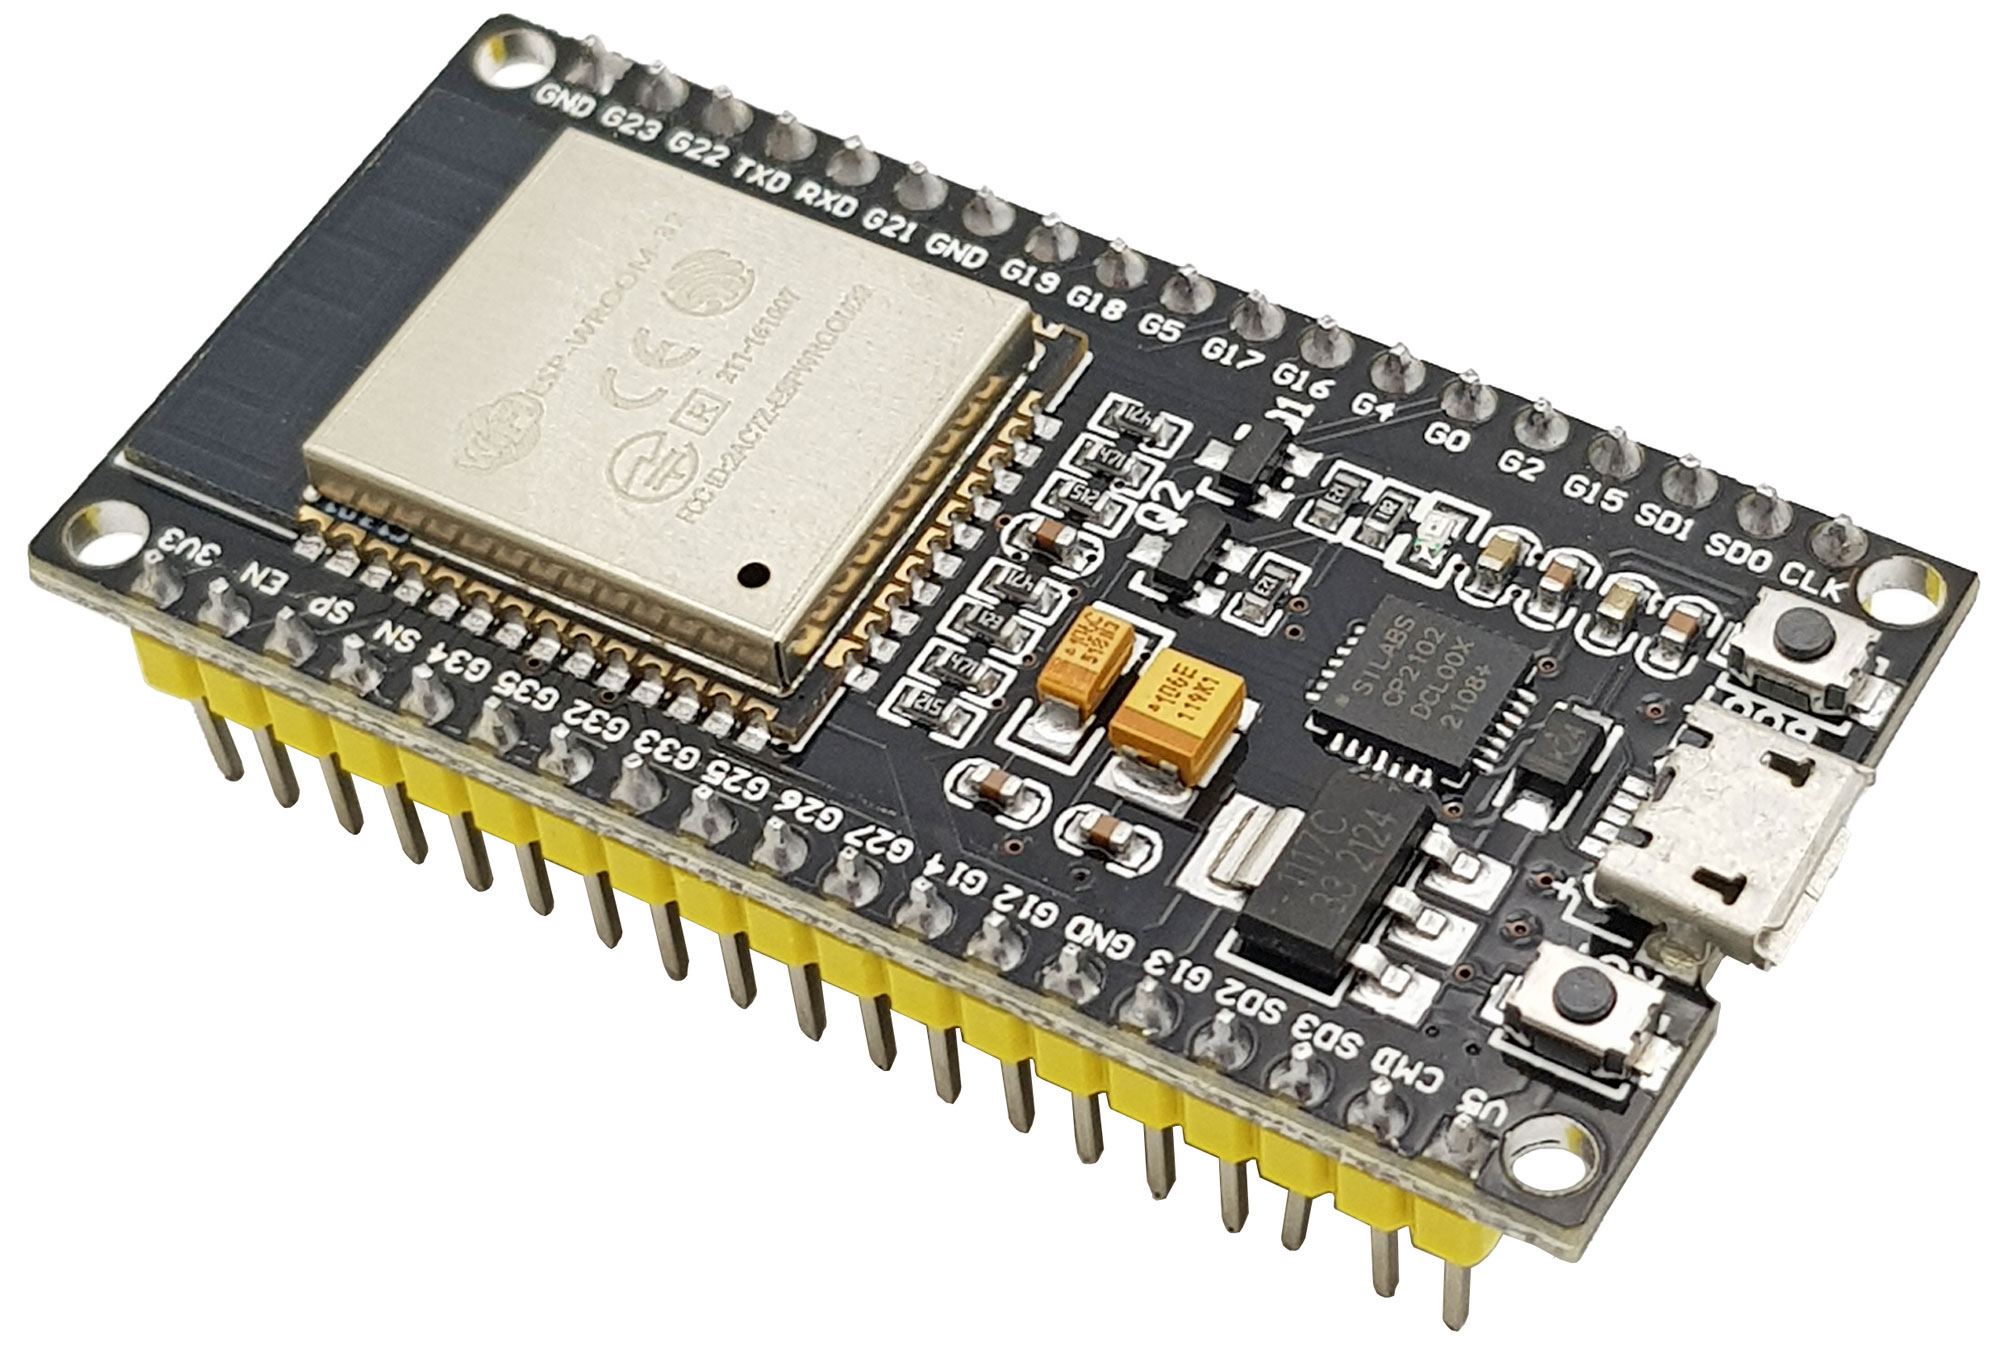
\includegraphics[width=\textwidth]{graphics/section2/ESP32.png}
                \caption*{Vi điều khiển ESP32}
            \end{subfigure}
            \caption*{}
        \end{figure}
        \end{itemize}
        
    \item \textbf{Vi điều khiển ESP32:} ESP32 là một vi điều khiển mạnh mẽ với khả năng kết nối Wi-Fi và Bluetooth. Trong dự án lần này, đây là bộ não của mạch.
    \newpage
    \item \textbf{Cảm biến dòng:} TA12 và TA17. Đây là 2 loại biến dòng được sử dụng để đo dòng điện qua mạch và gửi dữ liệu về vi điều khiển EPS32.
    \begin{figure}[h!]
        \centering
        % Ảnh trái 
        \begin{subfigure}{0.49\textwidth}
            \centering
            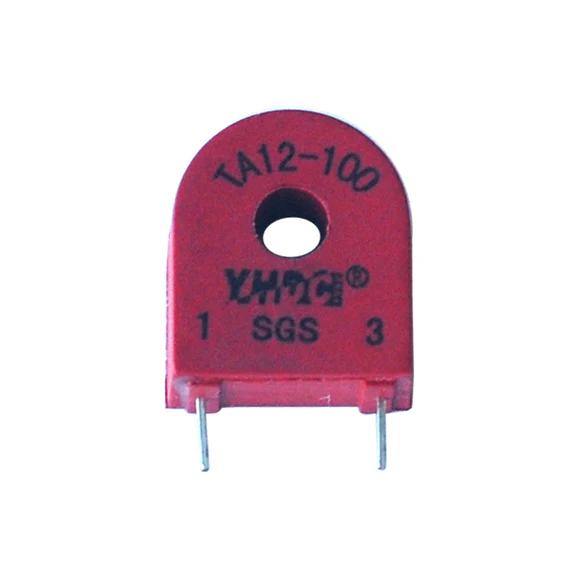
\includegraphics[width=0.5\textwidth]{graphics/section2/TA12.png}
            \caption*{TA12}
        \end{subfigure}
        \hfill
        % Ảnh phải
        \begin{subfigure}{0.49\textwidth}
            \centering
            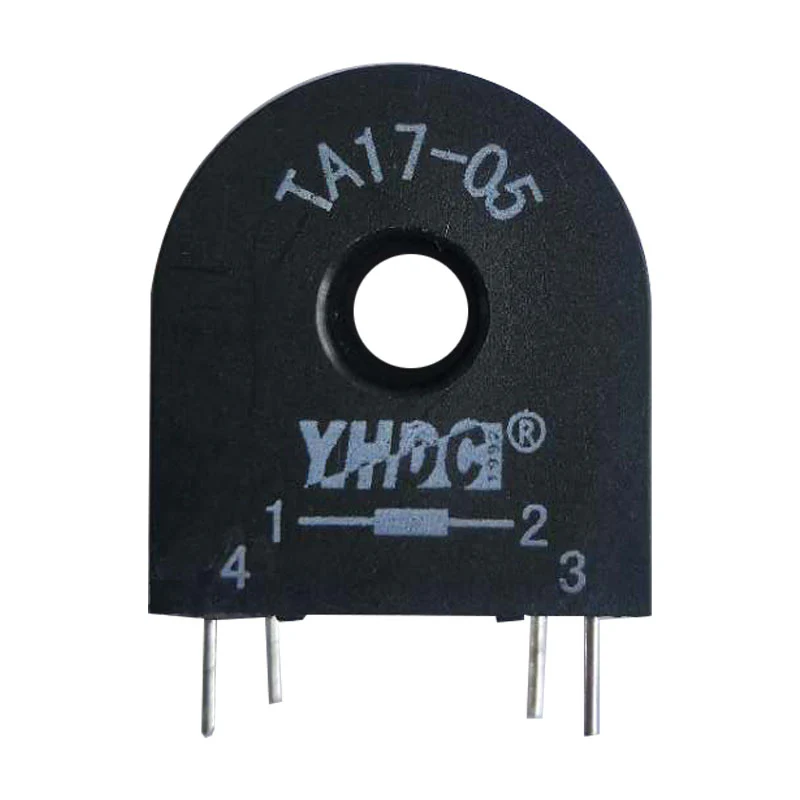
\includegraphics[width=0.46\textwidth]{graphics/section2/TA17.png}
            \caption*{TA17}
        \end{subfigure}
        \caption*{}
    \end{figure}
    \item \textbf{Các linh kiện khác:} Để gắn kết các linh kiện vừa kể trên với nhau, không thể không nhắc đến đầu nối và dây dẫn. Cuối cùng, nguồn điện là thứ cần thiết giúp cung cấp năng lượng cho toàn bộ linh kiện cho mạch, đảm bảo mạch thực hiện được chức năng như mong muốn của người thiết kế mạch. 
    
\end{itemize}
